% Copyright 2004 by Till Tantau <tantau@users.sourceforge.net>.
%
% In principle, this file can be redistributed and/or modified under
% the terms of the GNU Public License, version 2.
%
% However, this file is supposed to be a template to be modified
% for your own needs. For this reason, if you use this file as a
% template and not specifically distribute it as part of a another
% package/program, I grant the extra permission to freely copy and
% modify this file as you see fit and even to delete this copyright
% notice. 

\documentclass{beamer}
% There are many different themes available for Beamer. A comprehensive
% list with examples is given here:
% http://deic.uab.es/~iblanes/beamer_gallery/index_by_theme.html
% You can uncomment the themes below if you would like to use a different
% one:
%\usetheme{AnnArbor}
%\usetheme{Antibes}
%\usetheme{Bergen}
%\usetheme{Berkeley}
%\usetheme{Berlin}
%\usetheme{Boadilla}
%\usetheme{boxes}
%\usetheme{CambridgeUS}
%\usetheme{Copenhagen}
%\usetheme{Darmstadt}
\usetheme{default}
%\usetheme{Frankfurt}
%\usetheme{Goettingen}
%\usetheme{Hannover}
%\usetheme{Ilmenau}
%\usetheme{JuanLesPins}
%\usetheme{Luebeck}
%\usetheme{Madrid}
%\usetheme{Malmoe}
%\usetheme{Marburg}
%\usetheme{Montpellier}
%\usetheme{PaloAlto}
%\usetheme{Pittsburgh}
%\usetheme{Rochester}
%\usetheme{Singapore}
%\usetheme{Szeged}
%\usetheme{Warsaw}

\usepackage{graphicx}

\title{Presentation Title}

% A subtitle is optional and this may be deleted
\subtitle{Optional Subtitle}

\author{Michi RAKOTONARIVO}
% - Give the names in the same order as the appear in the paper.
% - Use the \inst{?} command only if the authors have different
%   affiliation.

\institute[Universities of Somewhere and Elsewhere] % (optional, but mostly needed)
{
  LJK EDP
}
\date{End Feb  -  end Mars 2018}


\AtBeginSubsection[]
{
  \begin{frame}<beamer>{Outline}
    \tableofcontents[currentsection,currentsubsection]
  \end{frame}
}

% Let's get started
\begin{document}

\begin{frame}
  \titlepage 
\end{frame}

% Section and subsections will appear in the presentation overview
% and table of contents.

\begin{frame}{}
\begin{itemize}
   \item  Stationnary Shr\"odinger equation 
    \begin{center}
       $ H \psi(x) = E \psi(x) , x  \in \mathrm{R}$ ,
       $H= \Delta + V(x) $  \\
       V is a periodic potential, E spectrum
    \end{center}
    
    \item Bloch theorem 
        \begin{itemize}
            \item  eigenfunction 
                \begin{center}
                    $\psi_{n,k} = e^{ik.x} u_{n,k} , x \in \mathcal{C} , \ k \in \mathcal{B}$ 
                \end{center}
                $B$ is the first Brillouin zone and $\mathcal{C}$ primitive cell
            \item  $u_{n,k}$ eigenvectors (periodic functions)
    
                
        \end{itemize}
    
    \item 

    $ ( \frac{h^2 |k|^2 }{2m} - i \frac{h^2 k. \nabla }{m} - \frac{h^2 \Delta }{2m} + V) u_{n,k}  = E(k) u_{n,k}$

\end{itemize}
\end{frame}

\begin{frame}
\begin{itemize}
    \item eigenvalues $E_{n,k}$ are reals and positives: \\
    taking h=1 and  m=1 , V=0 
    ~~\\
    \begin{center}
        $E_{n,k} = \frac{k^2 + 4n^2 \pi^2 - 4kn\pi}{2}, n \in \mathrm{Z}$
    \end{center}
\end{itemize}
\end{frame}


\begin{frame}{Results: analytic (without potential) }
     \begin{figure}
        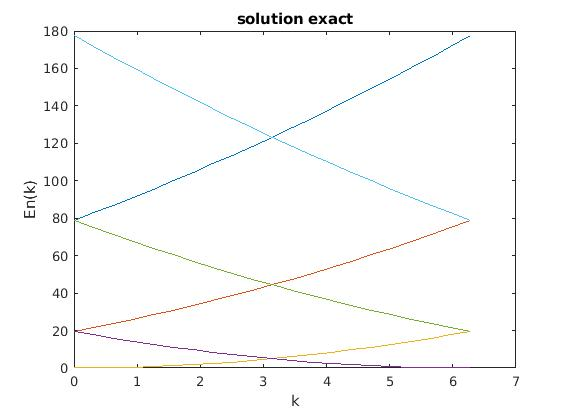
\includegraphics[width=6cm]{analytic.jpg} 
    \end{figure}
    
\end{frame}

\begin{frame}{Finite differences}
\begin{itemize}
    \item using central differencing scheme:
    \begin{center}
        $\nabla u \approx \frac{u_{j+1} - u_{j-1} }{ 2 \delta x}$ \\
        $\Delta u \approx \frac{u_{j+1} -2 u_j + u_{j-1} }{ \delta x^2} $
    \end{center}

    \item Shr\"odinger equation:

        $ E u_j  = \left( (  - \frac{ik}{2\delta x } -\frac{1}{2\delta x^2}) u_{j+1} + (\frac{ik}{2\delta x} - \frac{1}{2\delta x^2}) u_{j-1} + ( \frac{|k|^2}{2} + \frac{1}{\delta x^2} + V_j) u_j
        \right) $
\end{itemize}
\end{frame}
    
\begin{frame}{Finite differences}
Let $A= ( \frac{|k|^2}{2} + \frac{1}{\delta x^2} +V_j ) , B = (  - \frac{ik}{2\delta x } -\frac{1}{2\delta x^2} ), C = (\frac{ik}{2\delta x} - \frac{1}{2\delta x^2}) $ ~~\\ 
~~\\ 
N+1: number of points  \\
We notice a matrix M with dimension $NxN$, $M = \begin{bmatrix}
A  & B     & 0      &  \cdots      & 0     & C  \\
C  & A     & B      & \ddots &       & 0 \\
0 & C & A & B & \ddots &  \vdots  \\
\vdots   & \ddots & \ddots & \ddots & \ddots & 0  \\
0  &        & \ddots & C & A & B \\
B & 0      &   \cdots     & 0     & C      & A \\
\end{bmatrix}$

\end{frame}

\begin{frame}{Finite differences}

We have the following system :

$M  \begin{bmatrix}
u_0  \\
u_1  \\
\vdots   \\
\vdots  \\
u_{N-2}   \\
u_{N-1} \\
\end{bmatrix}
= E  \begin{bmatrix}
u_0  \\
u_1  \\
\vdots   \\
\vdots  \\
u_{N-2}   \\
u_{N-1} \\
\end{bmatrix}$

\end{frame}

\begin{frame}{Results: Finite differences }
V=0 and V= $10\cos(4 \pi x)$, number of points N=100

\begin{figure}
    \centering
    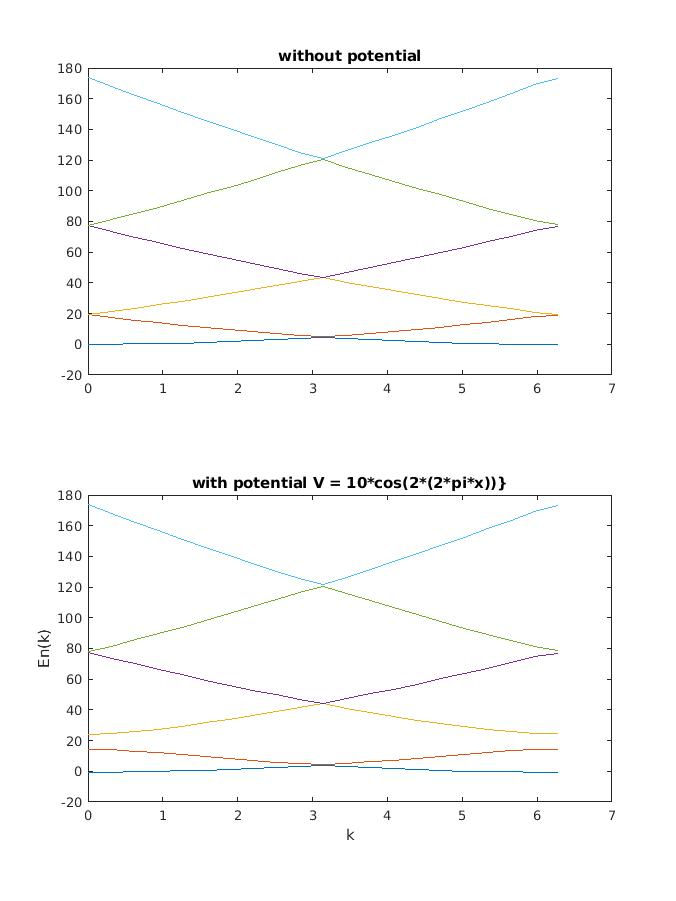
\includegraphics[width=5.5cm]{num_100.jpg} 
    \label{fig:my_label}
\end{figure}
\end{frame}


\begin{frame}{Results: Finite differences}
V=0 and V= $10\cos(4\pi x)$, number of points N=1000

\begin{figure}
    \centering
    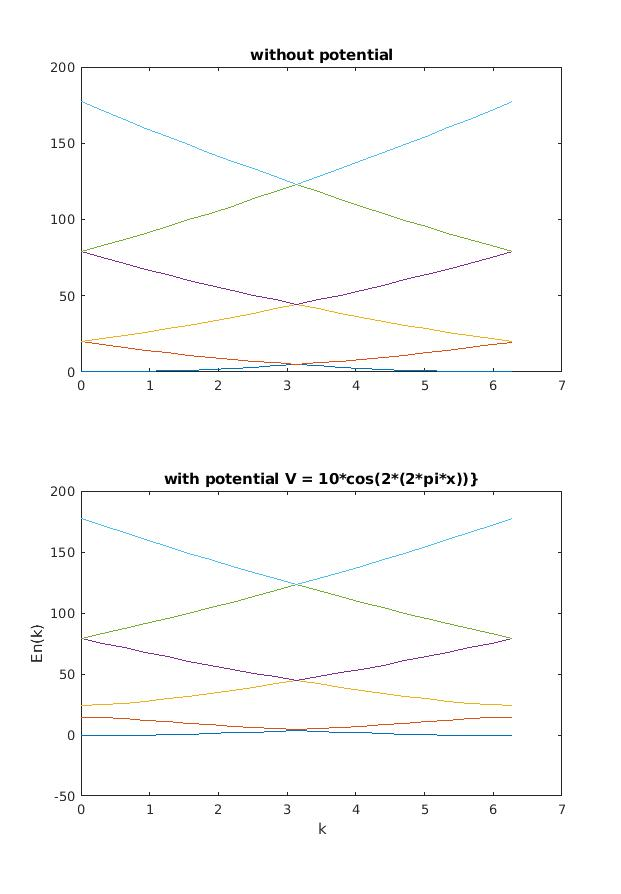
\includegraphics[width=5.5cm]{num_1000.jpg} 
    \label{fig:my_label}
\end{figure}
\end{frame}

\begin{frame}{Finite Element (V=0)}
    $\int \frac{ |k|^2 }{2} u v - i  k. \nabla u v + \frac{1}{2} \nabla u \nabla v    = E \int  u v $ \\
    \begin{itemize}
        \item space : $P1$  \\
        \item base: 
            \begin{center}
                $\phi_{i}(x) = \frac{1}{\delta x} (x - x_i) , x \in [x_i,x_{i+1}]$ \\
                $ \phi_{i+1}(x) = \frac{1}{\delta x} (x - x_i) , x \in [x_i,x_{i+1}] $
            \end{center}
            
            
        \item  Matrix $2x2$ : \\ 
            $\begin{bmatrix}
            \int_{x_{i}}^{x_{i+1}} a(\phi_{i},\phi_{i}) &  
            \int_{x_{i}}^{x_{i+1}} a(\phi_{i},\phi_{i+1}) \\
            \int_{x_{i}}^{x_{i+1}} a(\phi_{i+1},\phi_{i}) &  
            \int_{x_{i}}^{x_{i+1}} a(\phi_{i+1},\phi_{i+1})\\
            \end{bmatrix}
            = \frac{ |k|^2 }{2} 
            \begin{bmatrix}
            \frac{\delta x}{3} &  \frac{\delta x}{6} \\
            \frac{\delta x}{6} &  \frac{\delta x}{3} \\
            \end{bmatrix} 
            - ik 
            \begin{bmatrix}
            \frac{1}{2} &  \frac{1}{2}  \\
            \frac{-1}{2}  &  \frac{-1}{2}  \\
            \end{bmatrix}
            + \frac{1}{2} 
            \begin{bmatrix}
            \frac{1}{\delta x} &  \frac{-1}{\delta x}  \\
            \frac{-1}{\delta x}  &  \frac{1}{\delta x}  \\
            \end{bmatrix} 
            =
            \begin{bmatrix}
            A &  B  \\
            C &  A  \\
            \end{bmatrix}$
    \end{itemize}
~~\\
The dimension of the final matrix is $NxN$ 
\end{frame}

\begin{frame}{Finite Element (V=0)}
    Final system: \\
    $M_1 = \begin{bmatrix}
A  & B     & 0      &  \cdots      & 0     & C  \\
C  & A     & B      & \ddots &       & 0 \\
0 & C & A & B & \ddots &  \vdots  \\
\vdots   & \ddots & \ddots & \ddots & \ddots & 0  \\
0  &        & \ddots & C & A & B \\
B & 0      &   \cdots     & 0     & C      & A \\
\end{bmatrix}$

$M_2 = \begin{bmatrix}
\frac{\delta x}{3}  & \frac{\delta x}{6}    & 0      &  \cdots      & 0     & \frac{\delta x}{6} \\
\frac{\delta x}{6}  & \frac{\delta x}{3}      & \frac{\delta x}{6}      & \ddots &       & 0 \\
0 & \frac{\delta x}{6} & \frac{\delta x}{3} & \frac{\delta x}{6} & \ddots &  \vdots  \\
\vdots   & \ddots & \ddots & \ddots & \ddots & 0  \\
0  &        & \ddots & \frac{\delta x}{6} & \frac{\delta x}{3} & \frac{\delta x}{6} \\
\frac{\delta x}{6} & 0      &   \cdots     & 0     & \frac{\delta x}{6}      & \frac{\delta x}{3}  \\
\end{bmatrix} 
$ $\Longrightarrow M_1U = EM_2U$
\end{frame}
\begin{frame}{Results: finite element (V=0)}
$N=100(left), N=1000 (right)$
 \begin{figure}
    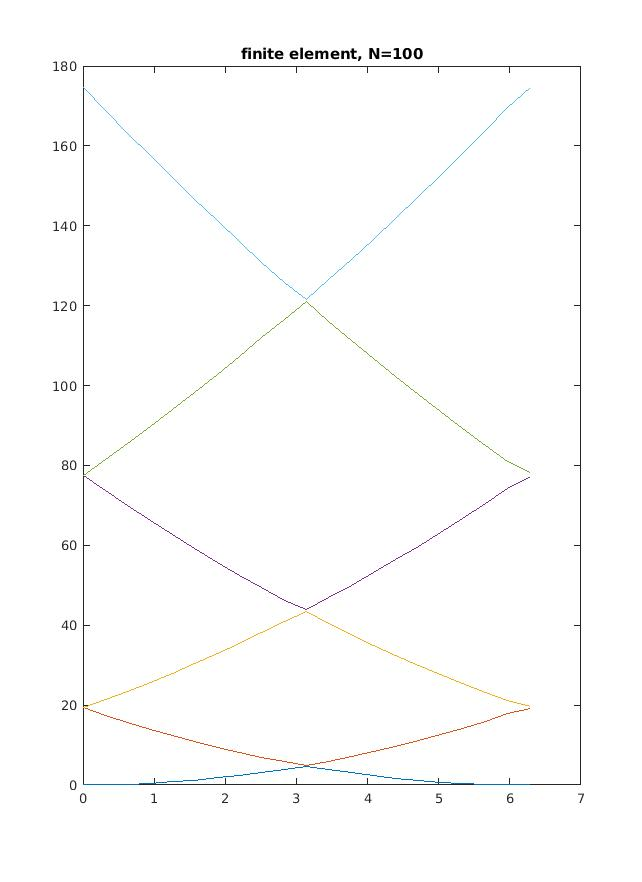
\includegraphics[width=4.8cm]{finite_100.jpg} 
    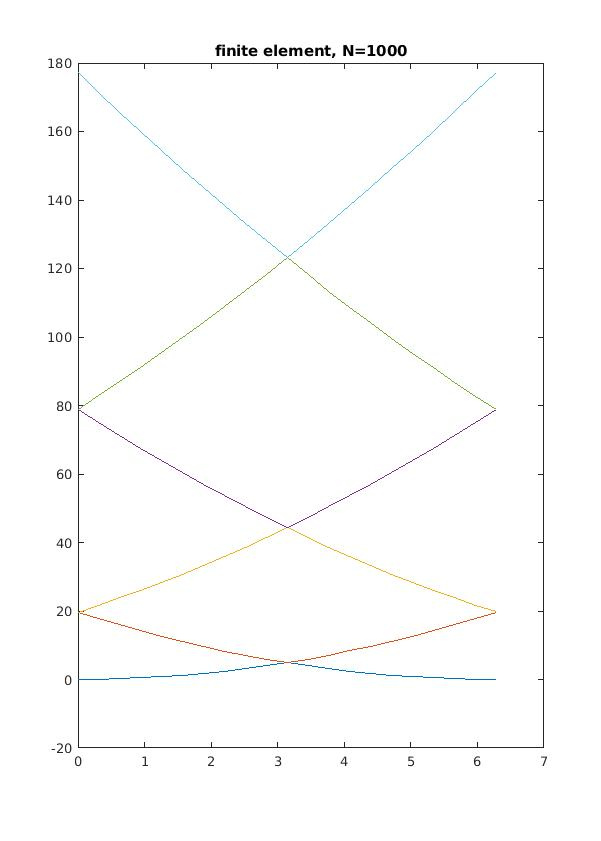
\includegraphics[width=4.7cm]{finite_1000.jpg}
\end{figure}   
\end{frame}


\begin{frame}{Errors: Finite element/Finite differences/Analytic (V=0)}
\begin{itemize}
    \item number of eigen values $nev = 6$
    \item k=0
    \item numbers of points: $N = 100(left) , N=500(right)$ 
\end{itemize}

 \begin{figure}
    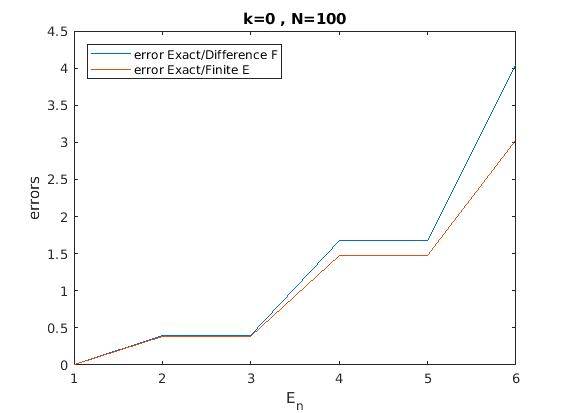
\includegraphics[width=5.5cm]{error_k0_100.jpg} 
    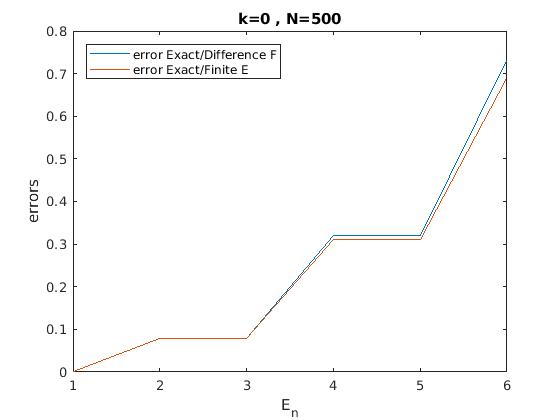
\includegraphics[width=5.5cm]{error_k0_500.jpg}
\end{figure} 
\end{frame}



\begin{frame}{Errors: Finite element/Finite differences/Analytic (V=0)}
\begin{itemize}
    \item N = 100, number of eigen values $nev=1 (6th)$, using Euclidean norm, $k=[0, 2\pi]$
\end{itemize}
 \begin{figure}
    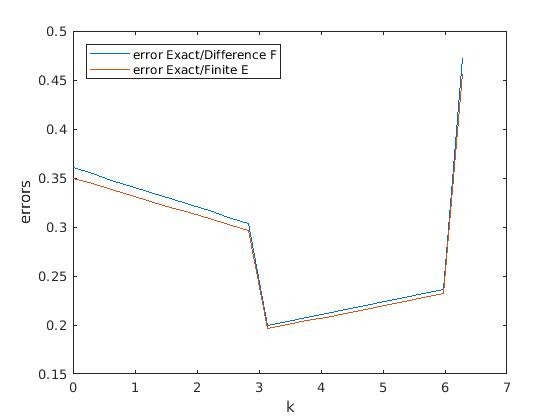
\includegraphics[width=6.6cm]{error_k0_6th_b.jpg} 
\end{figure} 
\end{frame}

\begin{frame}{Errors: Finite element/Finite differences/Analytic (V=0)}
\begin{itemize}
    \item N=1000,  number of eigen values $nev=[1,6]$, using Euclidean norm,, for $k=[0,2\pi]$
\end{itemize}
 \begin{figure}
    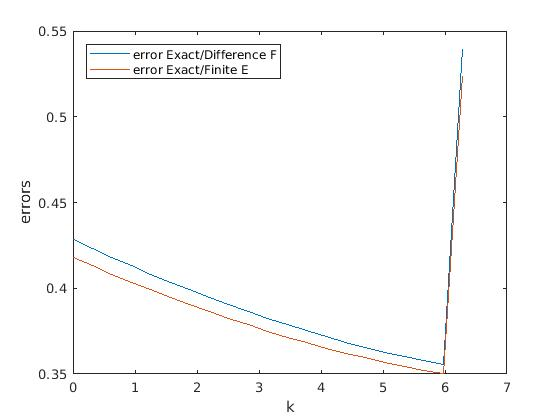
\includegraphics[width=6cm]{error_k.jpg}
\end{figure} 
\end{frame}


\begin{frame}{Errors: Finite element/Finite differences/Analytic (V=0)}
\begin{itemize}
    \item N=1000,  number of eigen values $nev=6$, using Euclidean norm,, for $k=[0,2\pi]$
\end{itemize}
 \begin{figure}
    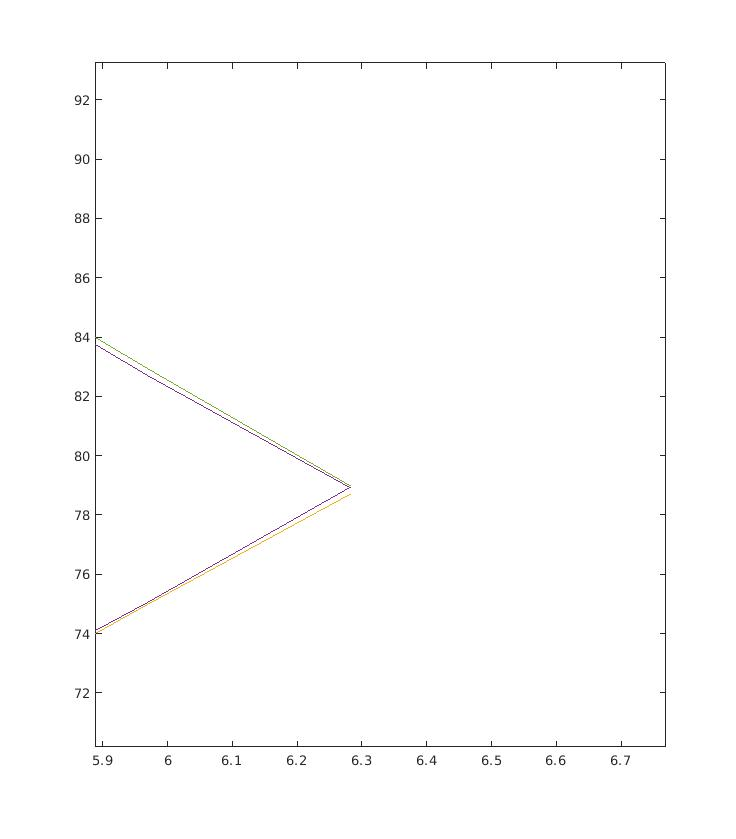
\includegraphics[width=5.5cm]{without_zoom_1.jpg}
    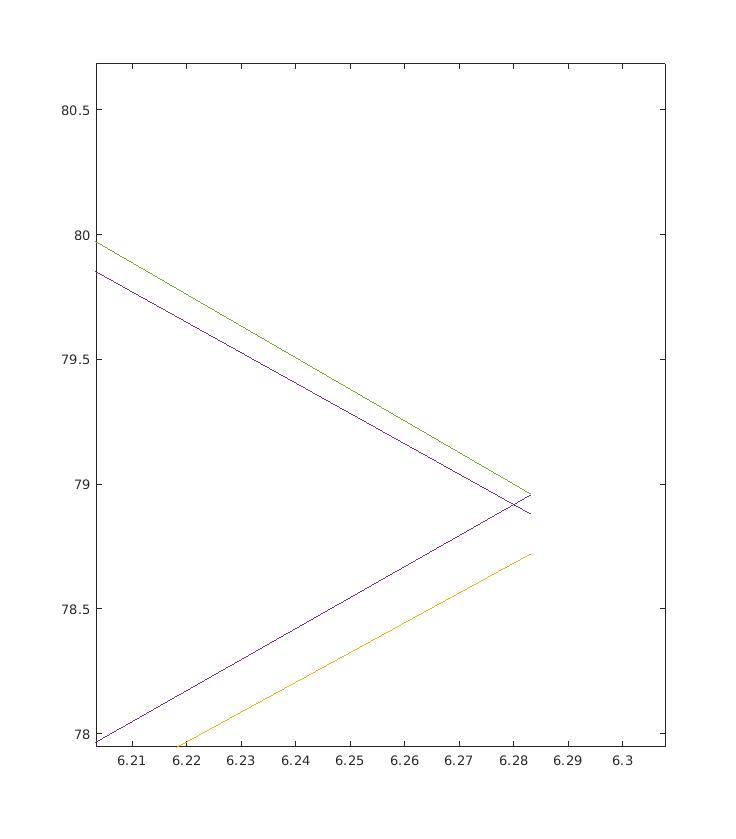
\includegraphics[width=5.5cm]{without_zoom_2.jpg} 
\end{figure} 
\end{frame}


\begin{frame}{Errors: Finite element/Finite differences/Analytic (V=0)}
    \begin{itemize}
        \item N = [100, 1000], number of eigen values $nev=1 (6th)$ , using Euclidean norm , $k=0$
    \end{itemize}

    \begin{figure}
    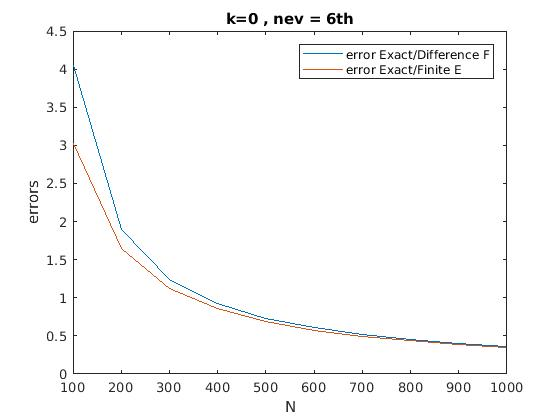
\includegraphics[width=5.5cm]{error_6th_k0.jpg} 
    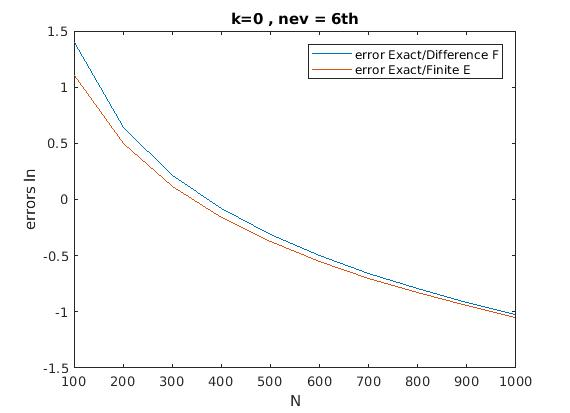
\includegraphics[width=5.5cm]{error_6th_k0_log.jpg} 
    \end{figure} 
\end{frame}





\begin{frame}{Errors: Finite element/Finite differences/Analytic (V=0)}
\begin{itemize}
    \item N = [100, 1000], number of eigen values $nev=6$, using Euclidean norm, k=0
\end{itemize}
 \begin{figure}
    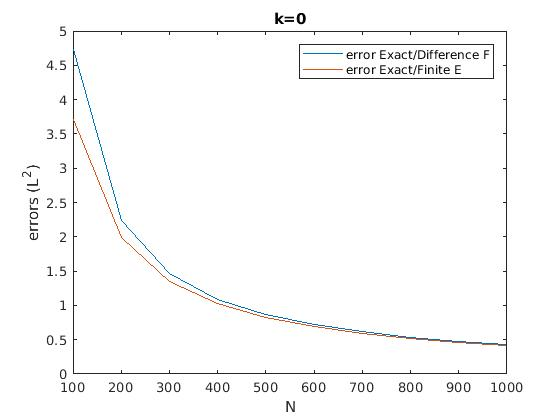
\includegraphics[width=6.6cm]{error_k0_N.jpg} 
\end{figure} 
\end{frame}


\begin{frame}{Errors: Finite element/Finite differences/Analytic (V=0)}
\begin{itemize}
    \item $dx=[\frac{1}{1000},\frac{1}{100}]$ ,  number of eigen values $nev=1 (6th) $, using Euclidean norm, for $k=[0,2\pi]$
    \item 6th (left), all 6 eigens values (right)
\end{itemize}
 \begin{figure}
    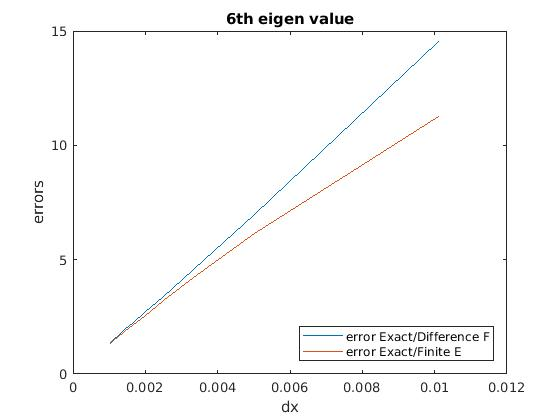
\includegraphics[width=6cm]{error_k_dx_6th.jpg} 
    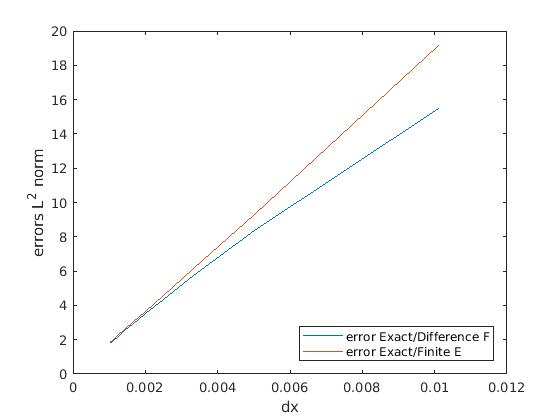
\includegraphics[width=6cm]{error_k_dx.jpg} 
\end{figure} 
\end{frame}



\begin{frame}{Errors: Finite element/Finite differences/Analytic (V= $10\cos(4 \pi x)$)}
    \begin{itemize}
        \item implementation of Finite element with potential
        \item comparison with finite differences
        \item compute exact solution with a giving potential and compare
    \end{itemize}
\end{frame}


\begin{frame}{Erreurs Exact/Differences/Element finis}
Pour $N=1000, k=[0,2\pi], E_6$
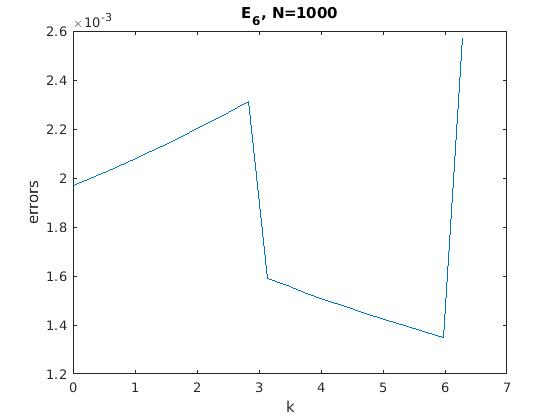
\includegraphics[width=6cm]{ERR_6_rel.jpg} 
 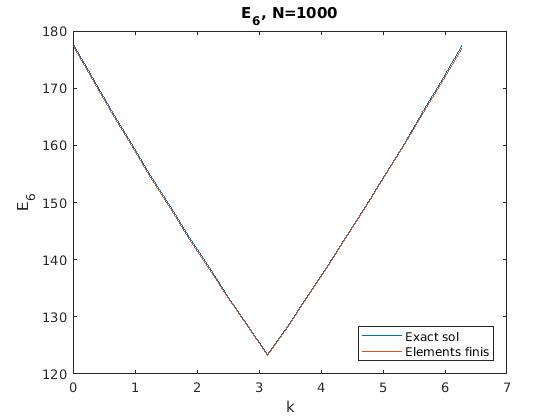
\includegraphics[width=6cm]{ERR_6_comp.jpg} 
\end{frame}

\begin{frame}{Erreurs Exact/Differences/Element finis}
Pour $N=1000, k=[0,2\pi], E_1$
   
\end{frame}

\end{document}



